\chapter{Measurement Procedure}
\section{Photon Pair Source}
\begin{figure}[H]
    \centering
    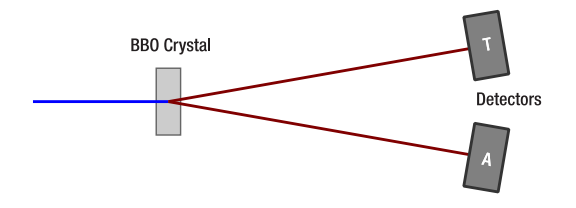
\includegraphics[width=70mm,scale=0.5]{Quantenoptik/include/A1.PNG}
    \caption{Schematic Setup for the Photon Pair Source} 
    \label{fig:A1}
\end{figure}
To test, if the source actually emits photon pairs, a setup like the one in figure \ref{fig:A1} is used. As already explained in the previous chapter, a pump laser generates a photon pair in a crystal, a barium borate (BBO) crystal. There are two single photon detectors, T and A, in each path that measure the count rates $R$ of the photons. To determine, whether the source really emits photon pairs, the second-order correlation function 
\begin{equation}
    g_{PS}^{(2)}(0)=\frac{R_\text{TA}}{R_\text{A}\cdot R_\text{T}\cdot \Delta t}
\end{equation}
needs to be calculated. $R_\text{A}$ and $R_\text{T}$ are the single detector rates of the detectors A and T, $R_\text{TA}$ is the coincidence count rate of both detectors and $\Delta t$ is the time window within photons are detected at both detectors simultaneously. 

\section{HBT Experiment with one Arm of the Pair Source}
\begin{figure}[H]
    \centering
    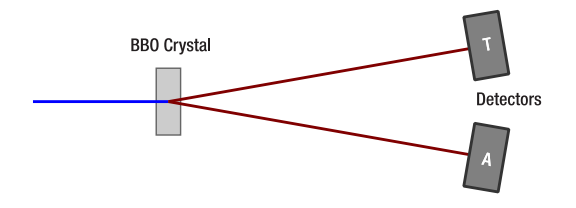
\includegraphics[width=70mm,scale=0.5]{Quantenoptik/include/A1.PNG}
    \caption{Schematic Setup for the HBT Experiment with one Arm of the Pair Source} 
    \label{fig:A2}
\end{figure}
The next experiment will be to test if one arm of the photon pair source is a single photon source. The setup is shown in figure \ref{fig:A2}. The detection arm leading to detector T is blocked with a screen. In the other path, there is a beamsplitter placed between the crystal and the detector A. At the outputs of the beamsplitter, there are two single photon detectors A and B. Once again the, the correlation function will be determined, but this time with the count rates of the detectors A and B. 

\section{Grangier-Roger-Aspect Experiment}
\label{GRA}
\begin{figure}[H]
    \centering
    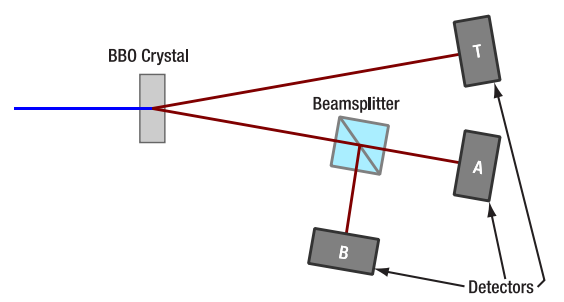
\includegraphics[width=70mm,scale=0.5]{Quantenoptik/include/A3.PNG}
    \caption{ Schematic Setup for the Grangier-Roger-Aspect Experiment} 
    \label{fig:A3}
\end{figure}
With the Grangier-Roger-Aspect Experiment one can find out, if the pair source is a single photon source when counts are measured only in coincidence with the trigger detector. The setup is the same as in the prior experiment but without the blocking screen. Now, the single count rate $R_\text{T}$ of detector T, the twofold coincidence count rates of detector T
with detectors A and B $R_\text{TA}, R_\text{TB}$  and triple coincidence count rate $R_\text{TAB}$ are being measured. With these values, 
\begin{equation}
    g_\text{GRA}^{(2)}(0)=\frac{R_\text{TAB}\cdot R_\text{T}}{R_\text{TA}\cdot R_\text{TB}}
    \label{eq:A3}
\end{equation}
can be calculated. 

\section{GRA Experiment with Classical Light}
\begin{figure}[H]
    \centering
    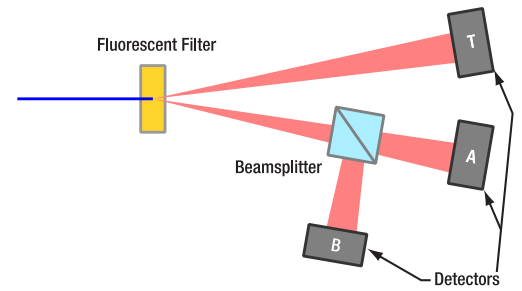
\includegraphics[width=70mm,scale=0.5]{Quantenoptik/include/A4.PNG}
    \caption{Schematic Setup for the GRA Experiment with Classical Light}
    \label{fig:A4}
\end{figure}
Next, the previous experiment will be performed again but with a non-pair source. Instead of the BBO crystal a fluorescent filter is now used, which emits fluorescent light in all directions. With same formla \ref{eq:A3} as before, the correlation can be calculated. 

\section{Malus’ Law for Single Photons}
\begin{figure}[H]
    \centering
    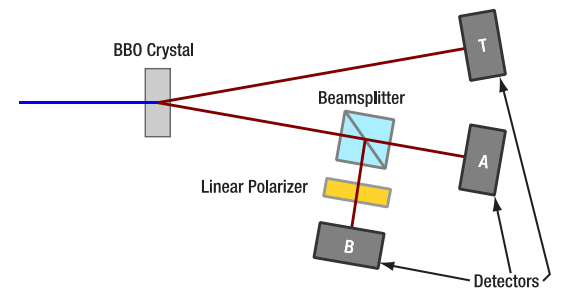
\includegraphics[width=70mm,scale=0.5]{Quantenoptik/include/A5.PNG}
    \caption{Schematic Setup for the Single Photon Malus’ Law Experiment}
    \label{fig:A5}
\end{figure} 
In the last experiment, the polarization properties of single photons will be tested. The setup is like the one in \ref{GRA} with a rotatable linear polarizer placed between the beamsplitter and detector B. For the measurement, the polarizer will be rotated by 10° and repeated from 0° to 180°. 
